%%%%%%%%%%%%%%%%%%%%%%%%%%%%%%%%%%%%%%%%%%%%%%%%%%%%%%%%%%%%%%%%%%%%%%%%
% Plantilla TFG/TFM
% Escuela Politécnica Superior de la Universidad de Alicante
% Realizado por: Jose Manuel Requena Plens
% Contacto: info@jmrplens.com / Telegram:@jmrplens
%%%%%%%%%%%%%%%%%%%%%%%%%%%%%%%%%%%%%%%%%%%%%%%%%%%%%%%%%%%%%%%%%%%%%%%%

\chapter{Resultados}
\label{resultados}



  En esta sección se detallarán los resultados de cada una de las etapas del proyecto y los experimentos finales para realizar un análisis comparativo entre ellos.


\section{Algoritmo Genético}

  En primer lugar analizaremos la evolución de los hiperparámetros del \glsentryshort{xgboost} gracias al algoritmo genético. En la figura \ref{EvolucionHiperparametrosImage} se pueden visualizar la evolución de los hiperparámetros del mejor individuo en cada generación a través del transcurso de interaciones. Se puede observar cómo el mejor individuo de cada generación va variando los tres hiperparámetros probando distintos valores hasta converger aproximadamente en la iteración \textit{21}.

  \begin{figure}[H]
      \centering
      \includesvg[scale=0.4]{archivos/5.Resultados/GA/EvolucionHiperparametros}
      \caption{Evolución de hiperparámetros a lo largo de las iteraciones.}
      \label{EvolucionHiperparametrosImage}
   \end{figure}

  \begin{figure}[H]
      \centering
      \includesvg[scale=0.4]{archivos/5.Resultados/GA/EvolucionF1Score}
      \caption{Evolución del macro F1 score a lo largo de las iteraciones.}
      \label{EvolucionF1ScoreImage}
   \end{figure}

  En la tabla \ref{BestGASolutionTable} se puede observar el mejor individuo obtenido después de \textit{50} generaciones.

  \begin{table}[H]
      \centering
          \begin{tabular}{ |c|c| } 
              \hline
              \textbf{Hiperparámetro} & \textbf{Valor}\\
              \hline
                  Profundidad Máxima & 1 \\
                  Peso mínimo de los hijos & 0.01 \\ 
                  ETA & 0.049 \\ 
              \hline

          \end{tabular}
      \caption{Mejores parámetros de XGBoost tras aplicar el algoritmo genético.}
      \label{BestGASolutionTable}
  \end{table}

\section{XGBoost}

  A continuación se mostrará la importancia de las clases calculada por \glsentryshort{xgboost} mediante los hiperparámetros obtenidos en la ejecución del algoritmo genético. En la figura \cite{FeatureWeightsImage} se puede observar un diagrama de barras en el que las características \textit{tipo de persona}, \textit{tipo de carretera} y \textit{sexo} son las que más han influido a la hora de entrenar el modelo \glsentryshort{xgboost}, obteniendo un peso de \textit{0.177}, \textit{0.127} y \textit{0.111} respectivamente. Se pueden consultar los pesos calculados de todas las características en la tabla \ref{PesosFinalesCaracteristicas}, en la que los pesos de las categorías padres es la suma de cada una de las características hijas.

  \begin{figure}[H]
      \centering
      \includesvg[scale = 0.6]{archivos/5.Resultados/XGBoost/FeatureWeights}
      \caption{Pesos asignados por XGboost a las características.}
      \label{FeatureWeightsImage}
   \end{figure}


  \begin{table}[H]
    \centering
    \begin{tabular}{ |c|c|c|c| }
         \hline
         \textbf{Categoría} & \textbf{Peso Categoría} & \textbf{Característica} & \textbf{Peso Característica}\\

         \hline
         \multirow{4}{*}{Accidente}   & \multirow{4}{*}{0.299}        & Coordenada X          & 0.071\\
                                      &                               & Coordenada Y          & 0.066\\
                                      &                               & Hora                  & 0.055\\
                                      &                               & Vehículos implicados  & 0.051\\
                                      &                               & Tipo de accidente     & 0.057\\

         \hline
         \multirow{2}{*}{Carretera}   & \multirow{2}{*}{0.187}        & Distrito              & 0.059\\      
                                      &                               & Tipo carretera        & 0.127\\

         \hline
         \multirow{1}{*}{Ambiente}    & \multirow{1}{*}{0.050}        & Estado meteorológico  & 0.050\\

         \hline
         \multirow{1}{*}{Vehículo}    & \multirow{1}{*}{0.070}        & Tipo de vehículo      & 0.070\\


         \hline
         \multirow{4}{*}{Conductor}   & \multirow{4}{*}{0.394}        & Tipo Persona          & 0.177\\
                                      &                               & Sexo                  & 0.111\\
                                      &                               & Rango Edad            & 0.050\\
                                      &                               & Positivo              & 0.056\\
         \hline

    \end{tabular}

    \caption{Cálculo de pesos de características y categorías mediante XGBoost (los valores se han redondeado en base a tres decimales).}
    \label{PesosFinalesCaracteristicas}
  \end{table}


\section{Matrices}

  En esta sección se mostrará el proceso que sigue una observación del dataset original tipificada hasta llegar a una matriz de características \ref{ProcesoMatriz}. En primer lugar, los valores de la muestra original \ref{ProcesoMatriz:MuestraTipificada} se normalizan según el criterio \glsentryshort{zsn} para pasar a ser una observación cuyos valores estan acotados en un rango en función de la distribución normal de cada característica en el dataset \ref{ProcesoMatriz:MuestraNormalizada}. El siguiente paso será posicionar cada uno de los valores de la muestra en la posición correspondiente de la matriz de acuerdo a los índices calculados en el paso anterior, de tal forma que servirán como entradas a las redes neuronales convolucionales \ref{ProcesoMatriz:Array}.

    \begin{figure}
        \centering
        \scriptsize

        \begin{subtable}{.2\textwidth}
          \centering
          \renewcommand{\arraystretch}{1.4}

          \csvautotabular{archivos/5.Resultados/Matrices/fatal_original.csv}
          \caption{Muestra de accidente tipificada.}
          \label{ProcesoMatriz:MuestraTipificada}
        \end{subtable}
        \hspace{13em}
        \begin{subtable}{.2\textwidth}
          \centering
          \renewcommand{\arraystretch}{1.4}

          \csvautotabular{archivos/5.Resultados/Matrices/fatal_normalized.csv}
          \caption{Muestra de accidente normalizada.}
          \label{ProcesoMatriz:MuestraNormalizada}
        \end{subtable}
        \vskip\baselineskip
        \begin{subtable}{.2\textwidth}
          \centering
          \captionsetup{width=0.8\textwidth}
          \renewcommand{\arraystretch}{1.1}

          \csvautotabular{archivos/5.Resultados/Matrices/fatal_matrix.csv}
          \caption{Muestra transformada en matriz de valores.}
          \label{ProcesoMatriz:Array}
        \end{subtable}
        \hspace{17em}
        \begin{subfigure}[b]{0.4\textwidth}
          \centering
          \includesvg[scale=0.6]{archivos/5.Resultados/Matrices/accidente_fatal}
          \caption{Muestra transformada en matriz de grises.}
          \label{ProcesoMatriz:VisualizacionDeMatriz}
        \end{subfigure}
      \caption{Proceso que sigue una muestra del conjunto de datos tipificada hasta llegar a una matriz.}
      \label{ProcesoMatriz}
      \end{figure}


  A modo de ejemplo se muestra en la figura \ref{TresClasesAccidentesMatrices} un accidente de cada clase transformados a su matriz correspondiente.

  \begin{figure}[H]
      \centering
      \begin{subfigure}[b]{0.3\textwidth}
        \centering
        \includesvg[scale=0.5]{archivos/5.Resultados/Matrices/accidente_leve}
        \caption{Accidente leve.}
        \label{TresClasesAccidentesMatrices:AccidenteLeveImage}
      \end{subfigure}
      \hspace{1em}
      \begin{subfigure}[b]{0.3\textwidth}
        \centering
        \includesvg[scale=0.5]{archivos/5.Resultados/Matrices/accidente_severo}
        \caption{Accidente severo.}
        \label{TresClasesAccidentesMatrices:AccidenteSeveroImage}
      \end{subfigure}
      \hspace{1em}
      \begin{subfigure}[b]{0.3\textwidth}
        \centering
        \includesvg[scale=0.5]{archivos/5.Resultados/Matrices/accidente_fatal}
        \caption{Accidente fatal.}
        \label{TresClasesAccidentesMatrices:AccidenteFatalImage}
      \end{subfigure}

    \caption{Tres clases de accidentes convertidos a matrices.}
    \label{TresClasesAccidentesMatrices}
  \end{figure}

\section{KNN}

  Se puede observar en la tabla \ref{BestParamsKNNGridSearchTable} los mejores parámetros para \textit{KNN} después de haber ejecutado \textit{Grid Search} sobre el conjunto de entrenamiento.\\

  \begin{table}[H]
      \centering
      \begin{tabular}{ |c|c| }
          \hline
          Atributo & Valor\\
          \hline
              Número de vecinos & 91 \\ 
              Tipo de distancia & Minkowski \\ 
          \hline
      \end{tabular}
      \caption{Mejores parámetros de KNN tras aplicar GridSearch.}
      \label{BestParamsKNNGridSearchTable}
  \end{table}





  El resultado de aplicar ambas técnicas da lugar a la representación en forma matricial de los accidentes, como se puede observar en la figura \ref{SampledImagesExampleImage}.



\section{Entrenamiento de modelos}

  A continuación se detallará una comparativa desde distintos puntos de vista de los resultados de los modelos. A nivel de rendimiento computacional se mostrarán los tiempos de entrenamiento. En lo que respecta a los resultados de predicción se analizarán las métricas de clasificación y matrices de confusión para los conjuntos de dato de entrenamiento y test. Para las redes neuronales además se mostrará la gráfica de evolución de la función de pérdida en base al Micro-F1Score para los datos de entrenamiento y test.

  \subsection{Tiempos de entrenamiento}

    En la figura \ref{TiemposEntrenamientoImage} se muestran los tiempos de entrenamiento empleados por los modelos. Hay que recalcar que el método \glsentryshort{knn}, al proyectar las muestras de entrenamiento en un espacio n-dimensional, no conlleva un entrenamiento como tal. Observando la gráfica se puede apreciar que el modelo que más tiempo de entrenamiento emplea es el \glsentryshort{svc} con 593 segundos, seguido de las red convolucionales de una y dos dimensiones con 287 y 259 segundos respectivamente y por último el clasificador \glsentryshort{gnb}, que debido a su naturaleza es el que menos tiempo emplea en entrenar con 0.02 segundos. 


    \begin{figure}[h]
      \centering
      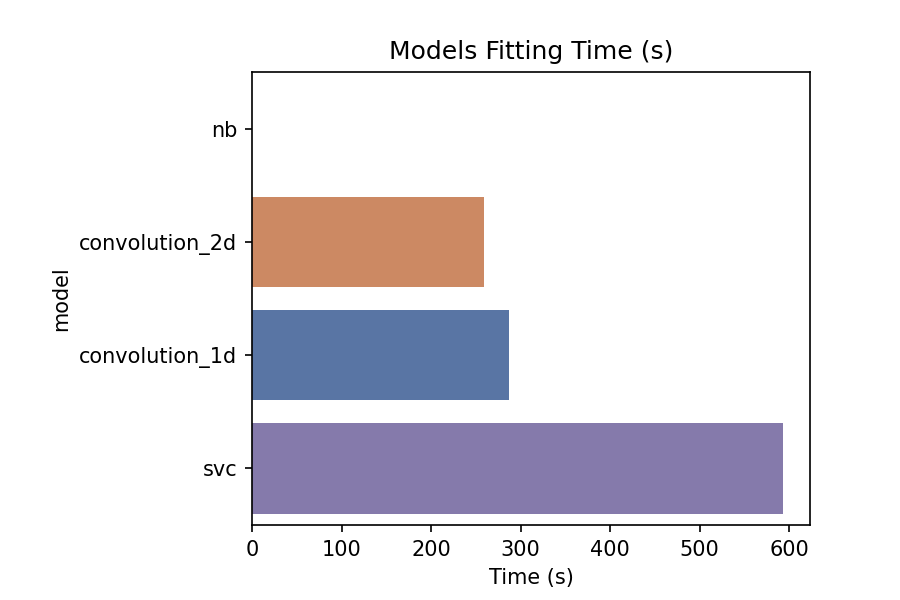
\includegraphics[width=12cm]{archivos/5.Resultados/TiemposEntrenamiento}
      \caption{Comparación entre los tiempos de entrenamiento de los modelos.}
      \label{TiemposEntrenamientoImage}
    \end{figure}


  
  \subsection{Gráficas de entrenamiento}


    En las figuras \ref{F1Score1DImage} y \ref{F1Score2DImage} podemos observar la evolución de la métrica definida a minimizar (Micro F1-score) en función de las 100 épocas que se ejecutarán para las redes convolucionales.


    Visualizando la gráfica de la convolucional de una dimensión \ref{F1Score1DImage} se puede comprobar que el Micro F1-score de entrenamiento va aumentando ligeramente a lo largo de las épocas sufriendo altibajos a medida que el modelo es entrenado, partiendo inicialmente desde \textbf{TODO: valor incial del Micro F1-score} hasta \textbf{TODO: valor final del Micro F1-score}. Observamos que los datos de validación \textbf{TODO: Describir en función de si entrenamos con los datos de validación smote-ii o con los de test}.

    \begin{figure}[h]
        \centering
        \includesvg[scale=0.3]{archivos/5.Resultados/CNN/1D/F1Score1D}
        \caption{Evolución de Micro F1-score sobre el conjunto de entrenamiento y validación CNN-1D.}
        \label{F1Score1DImage}
     \end{figure}

    En la siguiente figura \ref{F1Score2DImage} se puede apreciar que la tendencia del Micro F1-score \textbf{TODO: es más pronunciada....} con respecto a la convolución de una dimensión. Esto es debido a que ....... 

    \begin{figure}[h]
        \centering
        \includesvg[scale=0.3]{archivos/5.Resultados/CNN/2D/F1Score2D}
        \caption{Evolución de Micro F1-score sobre el conjunto de entrenamiento y validación CNN-2D.}
        \label{F1Score2DImage}
     \end{figure}


  \subsection{Reportes de clasificación}
       
    A continuación se mostrarán los reportes de clasificación resultantes de predecir los datos de entrenamiento con los que han aprendido los modelos. Este proceso es útil para entender qué han aprendido los modelos tras su ejecución, con la finalidad de observar cómo se clasifican cada una de las clases para cada uno. Como se puede observar, el modelo que peor resultados nos da visualizando el F1 score \textbf{TODO: el modelo}

    \begin{table}
        \scriptsize

        \begin{subtable}{.2\textwidth}
          \renewcommand{\arraystretch}{1.2}

          \csvautotabular{archivos/5.Resultados/CNN/1D/1DClassificationReportTrain.csv}
          \caption{Métricas de clasificación del conjunto de entrenamiento CNN-1D.}
          \label{CNN1DTrainMetrics}
        \end{subtable}
        \hspace{17em}
        \begin{subtable}{.2\textwidth}
          \renewcommand{\arraystretch}{1.2}

          \csvautotabular{archivos/5.Resultados/NB/NBClassificationReportTrain.csv}
          \caption{Métricas clasificación del conjunto de entrenamiento Naive Bayes.}
          \label{NBTrainMetrics}
        \end{subtable}
        \vskip\baselineskip

        \begin{subtable}{.2\textwidth}
          \centering
          \renewcommand{\arraystretch}{1.2}

          \csvautotabular{archivos/5.Resultados/SVC/SVCClassificationReportTrain.csv}
          \caption{Métricas clasificación del conjunto de entrenamiento SVC.}
          \label{SVCTrainDMetrics}
        \end{subtable}
        \hspace{17em}
        \begin{subtable}{.2\textwidth}
          \renewcommand{\arraystretch}{1.2}

          \csvautotabular{archivos/5.Resultados/KNN/KNNClassificationReportTrain.csv}
          \caption{Métricas clasificación del conjunto de entrenamiento KNN.}
          \label{KNNTrainMetrics}
        \end{subtable}

        \begin{subtable}{.2\textwidth}
          \centering
          \renewcommand{\arraystretch}{1.2}

          \csvautotabular{archivos/5.Resultados/CNN/2D/2DClassificationReportTrain.csv}
          \caption{Métricas clasificación del conjunto de entrenamiento CNN-2D.}
          \label{CNN2DTrainMetrics}
        \end{subtable}
    \end{table}

  \subsection{Matrices de confusión}

    Explicar las matrices de confusión con datos de \textbf{ENTRENAMIENTO.}

    \begin{figure*}
        \centering
        \begin{subfigure}[b]{0.4\textwidth}
            \centering
            \includesvg[scale=0.4]{archivos/5.Resultados/CNN/1D/1DConfusionMatrixTrain}
            \caption{Matriz de confusión de CNN-1D sobre entrenamiento.}
            \label{ConfusionMatrixTrainImages:1D}
        \end{subfigure}
        \hspace{3em}
        % Añadir el espacio deseado, si se deja la linea en blanco la siguiente subfigura ira en una nueva linea
        \begin{subfigure}[b]{0.4\textwidth}
            \centering
            \includesvg[scale=0.4]{archivos/5.Resultados/CNN/2D/2DConfusionMatrixTrain}
            \caption{Matriz de confusión de CNN-2D sobre entrenamiento.} 
            \label{ConfusionMatrixTrainImages:2D}
        \end{subfigure}
        \vskip\baselineskip
        \begin{subfigure}[b]{0.4\textwidth}
            \centering
            \includesvg[scale=0.4]{archivos/5.Resultados/NB/NBConfusionMatrixTrain}
            \caption{Matriz de confusión de NB sobre entrenamiento.}
            \label{ConfusionMatrixTrainImages:NB}
        \end{subfigure}
        \hspace{3em}
        \begin{subfigure}[b]{0.4\textwidth}
            \centering
            \includesvg[scale=0.4]{archivos/5.Resultados/KNN/KNNConfusionMatrixTrain}
            \caption{Matriz de confusión de KNN sobre entrenamiento.}
            \label{ConfusionMatrixTrainImages:KNN}
        \end{subfigure}
        \vskip\baselineskip
        \begin{subfigure}[b]{0.4\textwidth}
            \centering
            \includesvg[scale=0.4]{archivos/5.Resultados/SVC/SVCConfusionMatrixTrain}
            \caption{Matriz de confusión de SVC sobre entrenamiento.}
            \label{ConfusionMatrixTrainImages:SVC}
        \end{subfigure}

        \caption{Matrices de confusión de los modelos sobre el conjunto de entrenamiento.}
        \label{ConfusionMatrixTrainImages}
     \end{figure*}


  \subsection{Comparativa entre modelos}

  En la figura \ref{ResultsTrainImage} se muestra gráficamente el rendimiento de cada modelo sobre el conjunto de entrenamiento, las métricas utilizadas son la precisión, sensitividad y el F1-score.

  Como podemos observar, los modelos predicen bien los datos de con los que han sido entrenados, esta primera clasificación nos da una idea de cómo han evaluado los modelos las muestras. Sin embargo, unos resultados prometedores sobre este conjunto no implican un buen rendimiento, el objetivo es la predicción de datos futuros que puedan llegar al modelo, por lo tanto, comprobaremos la calidad mediante el conjunto de test.

  \begin{figure}[h]
      \centering
      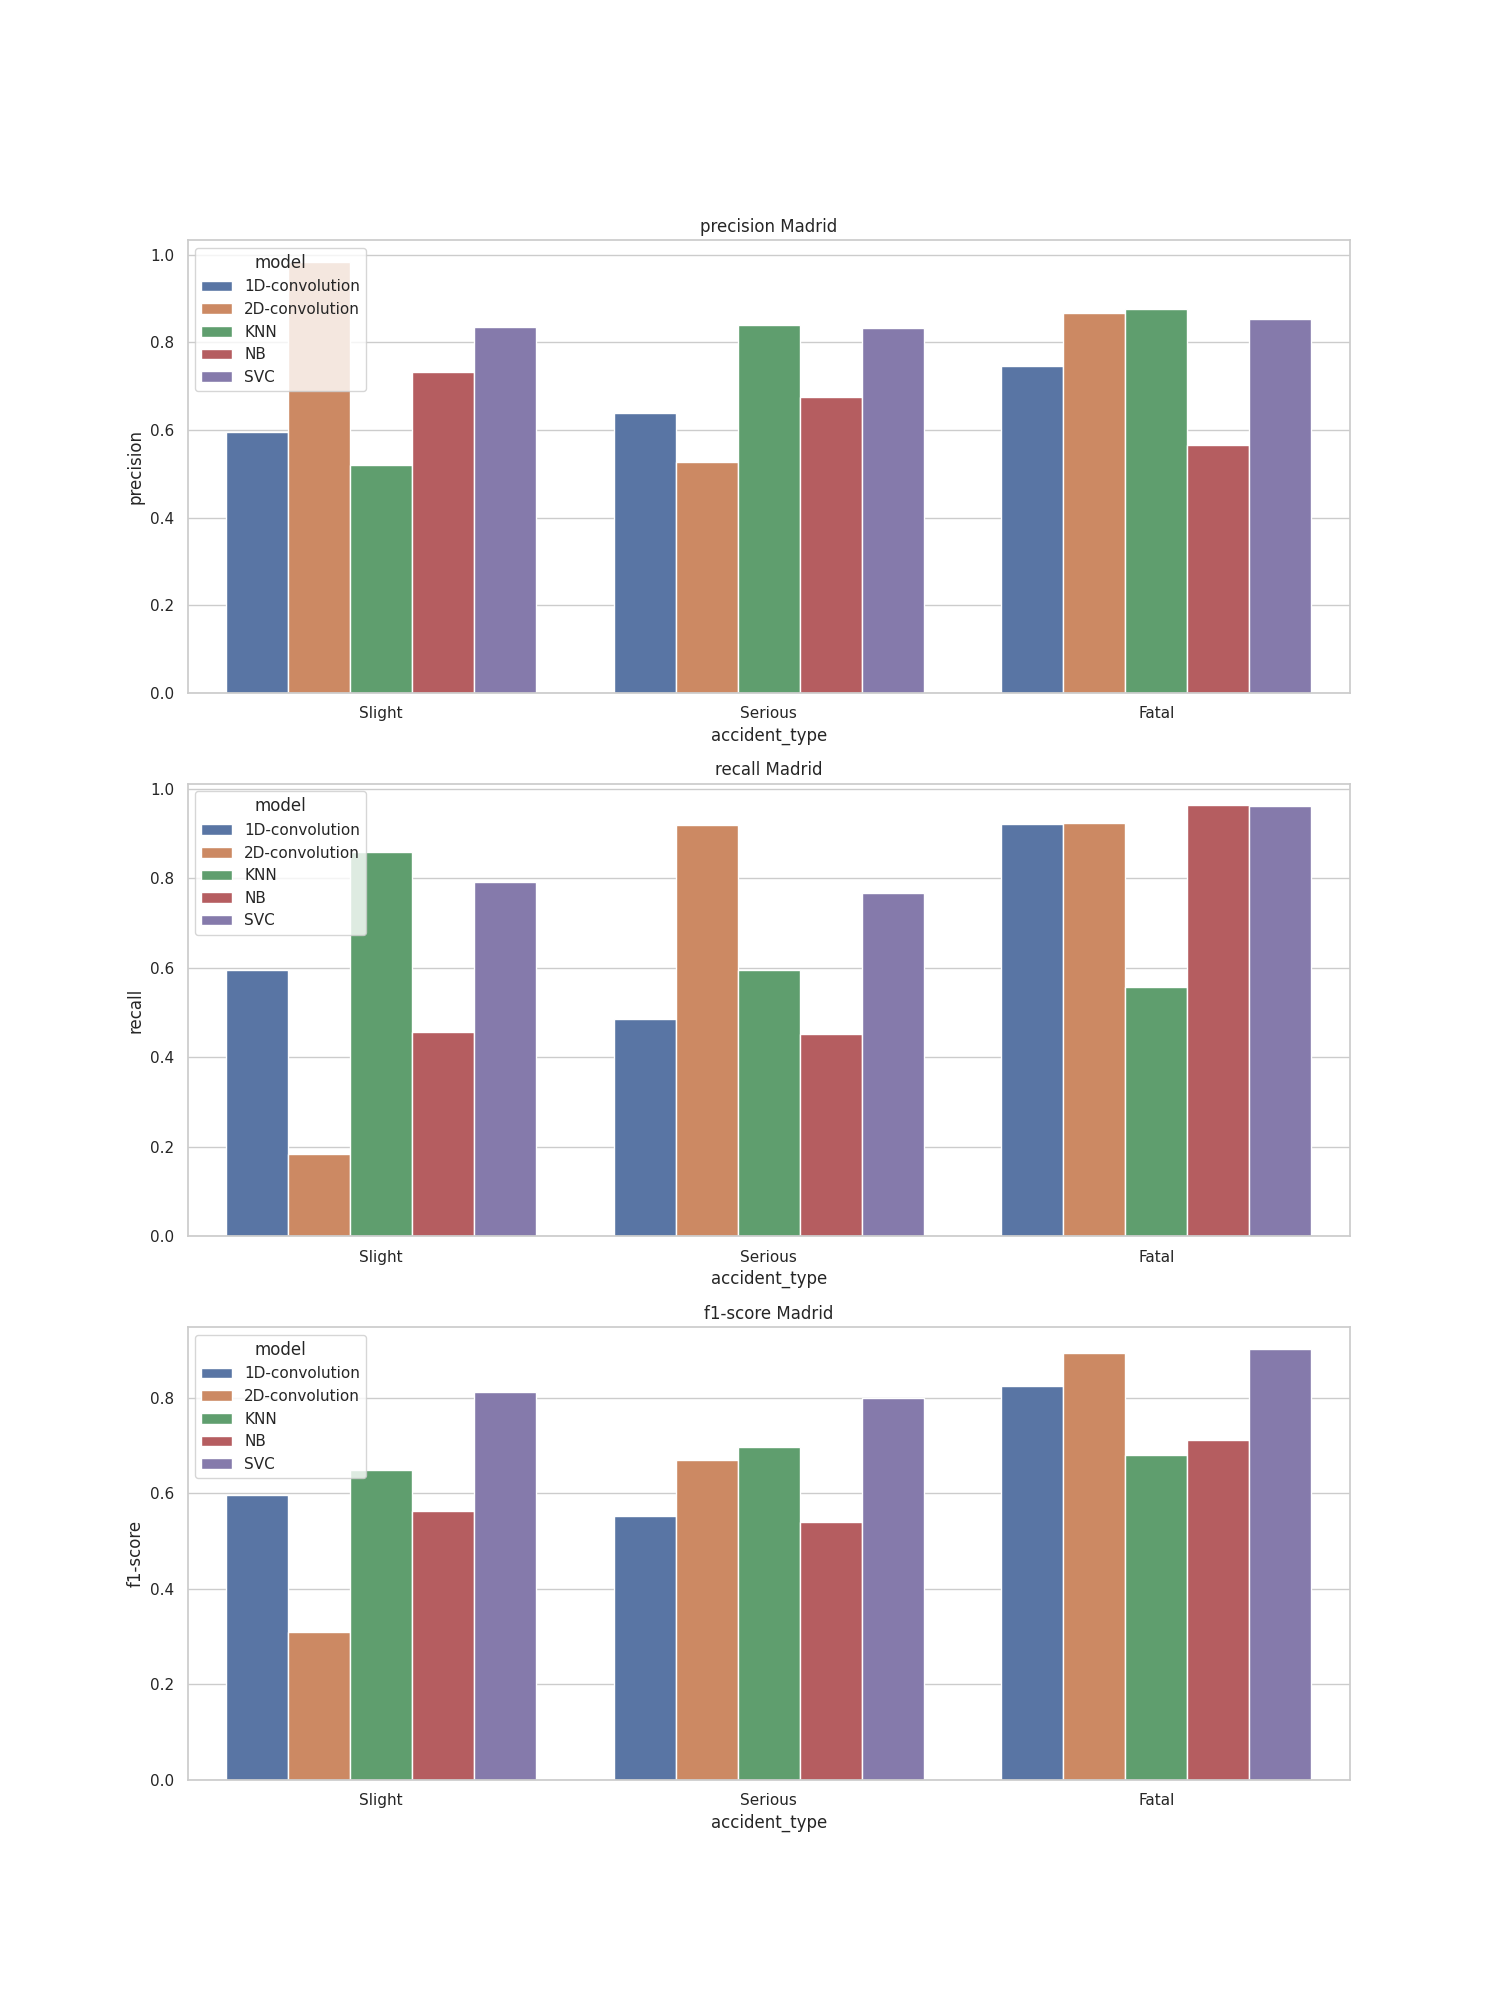
\includegraphics[width=16cm]{archivos/5.Resultados/ComparativaTrain}
      \caption{Comparativa de las métricas de las predicciones sobre el conjunto de entrenamiento de los modelos.}
      \label{ResultsTrainImage}
   \end{figure}



\section{Predicciones de modelos}

  \subsection{Reportes de clasificación}

    Explicar los reportes de clasificación con datos de \textbf{TEST.}

    \begin{table}
        \scriptsize

        \begin{subtable}{.2\textwidth}
          \renewcommand{\arraystretch}{1.2}

          \csvautotabular{archivos/5.Resultados/CNN/1D/1DClassificationReportTest.csv}
          \caption{Métricas de clasificación de test CNN-1D.}
          \label{CNN1DTestMetrics}
        \end{subtable}
        \hspace{17em}
        \begin{subtable}{.2\textwidth}
          \renewcommand{\arraystretch}{1.2}

          \csvautotabular{archivos/5.Resultados/NB/NBClassificationReportTest.csv}
          \caption{Métricas clasificación de test Naive Bayes.}
          \label{NBTestMetrics}
        \end{subtable}
        \vskip\baselineskip

        \begin{subtable}{.2\textwidth}
          \centering
          \renewcommand{\arraystretch}{1.2}

          \csvautotabular{archivos/5.Resultados/SVC/SVCClassificationReportTest.csv}
          \caption{Métricas clasificación de test SVC.}
          \label{SVCDTestMetrics}
        \end{subtable}
        \hspace{17em}
        \begin{subtable}{.2\textwidth}
          \renewcommand{\arraystretch}{1.2}

          \csvautotabular{archivos/5.Resultados/KNN/KNNClassificationReportTest.csv}
          \caption{Métricas clasificación de test KNN.}
          \label{KNNTestMetrics}
        \end{subtable}

        \begin{subtable}{.2\textwidth}
          \centering
          \renewcommand{\arraystretch}{1.2}

          \csvautotabular{archivos/5.Resultados/CNN/2D/2DClassificationReportTest.csv}
          \caption{Métricas clasificación de test CNN-2D.}
          \label{CNN2DTestMetrics}
        \end{subtable}
    \end{table}

  \subsection{Matrices de confusión}

    
    \ref{ConfusionMatrixTestImages}

    \begin{figure*}
        \centering
        \begin{subfigure}[b]{0.4\textwidth}
            \centering
            \includesvg[scale=0.4]{archivos/5.Resultados/CNN/1D/1DConfusionMatrixTest}
            \caption{Matriz de confusión de CNN-1D sobre test.}
            \label{ConfusionMatrixTestImages:1D}
        \end{subfigure}
        \hspace{3em}
        % Añadir el espacio deseado, si se deja la linea en blanco la siguiente subfigura ira en una nueva linea
        \begin{subfigure}[b]{0.4\textwidth}
            \centering
            \includesvg[scale=0.4]{archivos/5.Resultados/CNN/2D/2DConfusionMatrixTest}
            \caption{Matriz de confusión de CNN-2D sobre test.} 
            \label{ConfusionMatrixTestImages:2D}

        \end{subfigure}
        \vskip\baselineskip
        \begin{subfigure}[b]{0.4\textwidth}
            \centering
            \includesvg[scale=0.4]{archivos/5.Resultados/NB/NBConfusionMatrixTest}
            \caption{Matriz de confusión de NB sobre test.}
            \label{ConfusionMatrixTestImages:NB}
        \end{subfigure}
        \hspace{3em}
        \begin{subfigure}[b]{0.4\textwidth}
            \centering
            \includesvg[scale=0.4]{archivos/5.Resultados/KNN/KNNConfusionMatrixTest}
            \caption{Matriz de confusión de KNN sobre test.}
            \label{ConfusionMatrixTestImages:KNN}
        \end{subfigure}
        \vskip\baselineskip
        \begin{subfigure}[b]{0.4\textwidth}
            \centering
            \includesvg[scale=0.4]{archivos/5.Resultados/SVC/SVCConfusionMatrixTest}
            \caption{Matriz de confusión de SVC sobre test.}
            \label{ConfusionMatrixTestImages:SVC}
        \end{subfigure}

        \caption{Matrices de confusión de los modelos sobre el conjunto de test.}
        \label{ConfusionMatrixTestImages}
     \end{figure*}

  \subsection{Comparativa entre modelos}

    Explicar la comparativa de modelos con datos de \textbf{ENTRENAMIENTO.}

ninguno de los modelos aplicados es capaz de generalizar bien sore el conjunto de datos de test sin smote
    \begin{figure}[h]
        \centering
        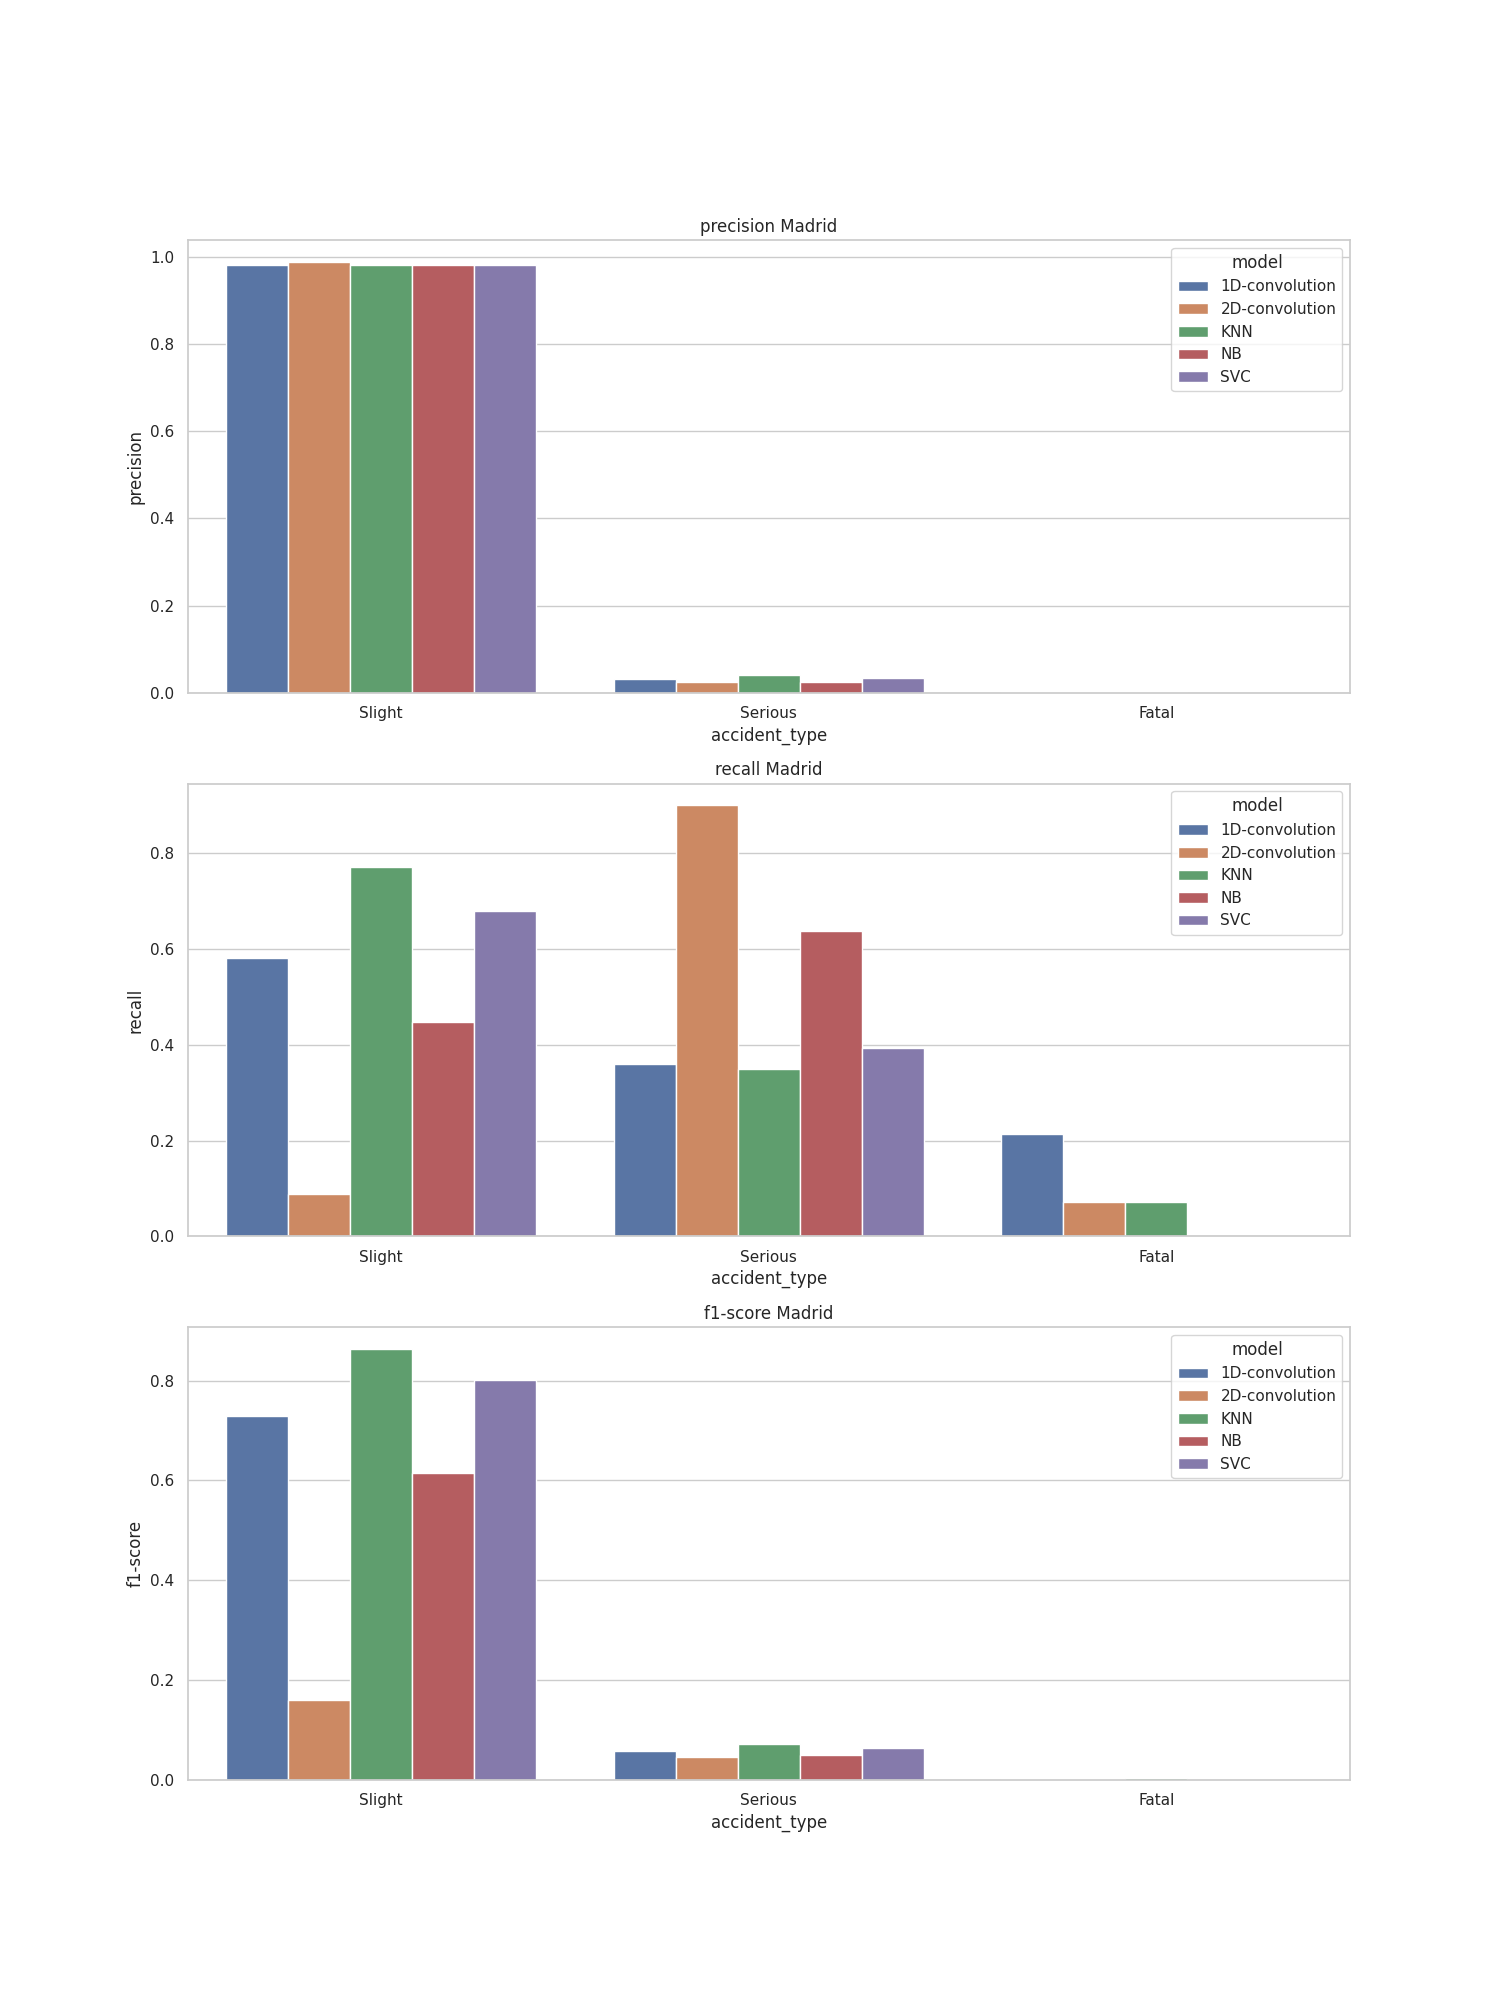
\includegraphics[width=16cm]{archivos/5.Resultados/ComparativaTest}
        \caption{Comparativa de las métricas de las predicciones sobre el conjunto de test de los modelos.}
        \label{ResultsTestImage}
     \end{figure}





ya sea porque el modelo está sobreajustado o por


Es importante recalcar que los resultados de estas predicciones están muy condicionados al tratamiento y las transformaciones de los datos.




 de la informacio que tenemos y de el tipo de limpieza que se ha hecho. Se ppodria hacer un estudio del valor numerico que se le asigna a cada variable en la limpieza, ya que seguramente al estar nosotros haciendolo aleatoriamente seguramente se esté creando algún patrón de jerarquía dentro de una columna o se le da mas importancia a un todoterreno que a un avion porque el todoterrento al tener un valor asignado más alto sera mas negro y por lo tanto la red predicira lo que sea



